\documentclass[a4paper,12pt]{report}

\newcommand{\nameInitial}{
    {F. Harraway}  %change colour to black and enter your initial and surname
}
\newcommand{\nameFull}{
  {Frank Harraway} %change colour to black and enter your firstname and surname
}
\newcommand{\stNumber}{
   {22623280} %change to black and enter your student number 
}
\newcommand{\myDate}{{\today} %change colour and if you want to date.
}
\newcommand{\signature}{frontmatter/fig/sig}   %Upload your signature as "frontmatter/fig/Signature.png"


%%%%%%%%%%%%%%%%%%%%%%%%%%%%%%%%%%%%%%%%%%%%%%%%%%%%%%%%%%%%%%%%%
%From here you can ignore up to \begin{document} (line 107)
%%%%%%%%%%%%%%%%%%%%%%%%%%%%%%%%%%%%%%%%%%%%%%%%%%%%%%%%%%%%%%%%%
% Page layout
\usepackage[left=2.2cm,right=2.2cm,top=2.2cm,bottom=2.2cm]{geometry}
% Figures
\usepackage[margin=\the\parindent,small,bf,sf]{caption}
\usepackage{graphicx}
\usepackage{pdfpages}
\setlength{\abovecaptionskip}{7.5pt}  % spacing above and below captions
\newcommand*{\WaterMark}[2][0.2\paperwidth]{\AddToShipoutPicture*{\AtTextCenter{\parbox[c]{0pt}{\makebox[0pt][c]{\includegraphics[width=#1]{#2}}}}}}
\usepackage{subcaption}
% Font and text
\usepackage[afrikaans,english]{babel}
\usepackage{microtype}
\usepackage{setspace}
\usepackage{lmodern}
\newcommand{\myemph}[1]{{\sffamily\bfseries#1}}
\sloppy
\onehalfspacing
\usepackage{siunitx}
\usepackage{lipsum}
% Headings
\usepackage[raggedright,sf,bf]{titlesec}
\titlelabel{\thetitle.\ }
\titleformat{\chapter}[display]{\huge\bfseries\sffamily}{\chaptertitlename\ \thechapter}{15pt}{\raggedright}
% \titleformat{\chapter}[display]{\centering\huge\bfseries\sffamily}{\chaptertitlename\ \thechapter:}{15pt}{}
\titlespacing*{\chapter}{0pt}{0pt}{10pt}  % remove spacing before chapter headings
% Table of contents
\makeatletter
\let\originall@chapter\l@chapter
\def\l@chapter#1#2{\originall@chapter{{\sffamily #1}}{#2}}
\makeatother
\let \savenumberline \numberline
\def \numberline#1{\savenumberline{#1.}}
% Mathematics
\usepackage[cmex10]{amsmath}
\usepackage{amssymb}
\usepackage{cancel}
\DeclareMathOperator*{\argmax}{arg\,max}
\newcommand{\T}{^\textrm{T}}
\newcommand{\tr}{\textrm{tr}}
\renewcommand{\vec}[1]{\boldsymbol{\mathbf{#1}}}
\newcommand{\defeq}{\triangleq}
% Tables
\usepackage{booktabs}
\usepackage{tabularx}
\usepackage{multirow}
\newcommand{\mytable}{
    \centering
    \small
    \renewcommand{\arraystretch}{1.2}
    }
\renewcommand{\tabularxcolumn}[1]{m{#1}}
\newcolumntype{C}{>{\centering\arraybackslash}X}
\newcolumntype{L}{>{\raggedright\arraybackslash}X}
% Header and footer
\usepackage{fancyhdr}
\pagestyle{fancy}
\fancyhf{}
\renewcommand{\sectionmark}[1]{\markright{\normalsize \thesection.\ #1}}
\fancyhead[C]{\nouppercase{\textit{\rightmark}}}
\fancyhead[RO]{\thepage}
% \fancyhead[LE]{\thepage}  % double-sided printing
\fancyfoot{}
\setlength\headheight{14.5pt}
\renewcommand{\headrulewidth}{0pt}
\fancypagestyle{plain}{\fancyhead{}
                       \renewcommand{\headrulewidth}{0pt}
                       \fancyfoot[C]{\thepage}}
% Pseudo-code
\usepackage{algorithm}  % should go before \usepackage{hyperref}
% Table of contents and hyperlinks
\usepackage{hyperref}
\hypersetup{colorlinks=true,linktoc=all,citecolor=black,linkcolor=black}
\usepackage[nottoc]{tocbibind}
% Pseudo-code
\usepackage{algpseudocode}  % should go after \usepackage{hyperref}
\renewcommand{\thealgorithm}{\arabic{chapter}.\arabic{algorithm}} 
\captionsetup[algorithm]{labelfont={bf,sf},font=small,labelsep=colon}
% Bibliography
\usepackage{cite}  % automatically reorder inline citations
\bibliographystyle{IEEEtran}
% Fix titlesec issue
\usepackage{etoolbox}
\makeatletter
\patchcmd{\ttlh@hang}{\parindent\z@}{\parindent\z@\leavevmode}{}{}
\patchcmd{\ttlh@hang}{\noindent}{}{}{}
\makeatother
 \usepackage[normalem]{ulem}
%%%%%%%%%%%%%%%%%%%%%%%%%%%%%%%%%%%%%%%%%%%%%%%%%%%%%%%%%%%%%%%%%
% Ignore up to here. 
%%%%%%%%%%%%%%%%%%%%%%%%%%%%%%%%%%%%%%%%%%%%%%%%%%%%%%%%%%%%%%%%%

\begin{document}

% Front matter
\graphicspath{{frontmatter/fig/}}
\pagenumbering{Alph}

\begin{titlepage}
\begin{center}


\includegraphics[width=10cm]{USlogo-top}

\vfill

{\sffamily \bfseries \huge E344 Assignment 6 \par}

\vfill

{\large {\Large \nameFull} \\ \stNumber \par}

\vfill

\vfill

{Report submitted in partial fulfilment of the requirements of the module \\
Design (E) 344 for the degree Baccalaureus in Engineering in the Department of
Electrical and Electronic Engineering at Stellenbosch University. \par}

\vfill

%{\large {Supervisor}: Dr L. Skywalker} %\\
% Department of Electrical and Electronic Engineering \par}

\vfill

{\Large \myDate}
\end{center}
\end{titlepage}

\pagenumbering{roman}
%\chapter*{Declaration}
\newpage
\pagestyle{plain}
\addcontentsline{toc}{chapter}{Declaration}
\makeatletter\@mkboth{}{Declaration}\makeatother

\centerline{
\includegraphics[width=8cm]{USlogo-top}}
\vspace*{-10pt}

\section*{\centering Plagiaatverklaring / \textit{Plagiarism Declaration}}

\vspace*{5pt}

\begin{enumerate}
    \item Plagiaat is die oorneem en gebruik van die idees, materiaal en ander intellektuele eiendom van ander persone asof dit jou eie werk is.\\
    \textit{Plagiarism is the use of ideas, material and other intellectual property of another's work
        and to present is as my own.}
    
    \item Ek erken dat die pleeg van plagiaat 'n strafbare oortreding is aangesien dit 'n vorm van diefstal is.\\
    \textit{I agree that plagiarism is a punishable offence because it constitutes theft.}
    
    \item Ek verstaan ook dat direkte vertalings plagiaat is. \\
    \textit{I also understand that direct translations are plagiarism.}
    
    \item Dienooreenkomstig is alle aanhalings en bydraes vanuit enige bron (ingesluit die internet) volledig verwys (erken). Ek erken dat die woordelikse aanhaal van teks sonder aanhalingstekens (selfs al word die bron volledig erken) plagiaat is. \\
    \textit{Accordingly all quotations and contributions from any source whatsoever (including the internet) have been cited fully. I understand that the reproduction of text without quotation marks (even when the source is cited) is plagiarism}
    
    \item Ek verklaar dat die werk in hierdie skryfstuk vervat, behalwe waar anders aangedui, my eie oorspronklike werk is en dat ek dit nie vantevore in die geheel of gedeeltelik ingehandig het vir bepunting in hierdie module/werkstuk of 'n ander module/werkstuk~nie. \\
    \textit{I declare that the work contained in this assignment, except where otherwise stated, is my original work and that I have not previously (in its entirety or in part) submitted it for grading in this module/assignment or another module/assignment.}
\end{enumerate}

\vfill

\noindent \begin{tabularx}{1.0\linewidth}{|L|L|}
    \hline
    \hspace{2cm} \large{\stNumber}& \vspace{4mm}\hspace{2cm} \includegraphics[height=1.5cm]{\signature}\\

    \vspace{0mm}{Studentenommer / \textit{Student number}} & \vspace{0mm} {Handtekening / \textit{Signature}} \\
    \hline
    \vspace{1mm}  \hspace{2cm} \large{\nameInitial} & \vspace{1mm} \hspace{2cm} \large{\myDate }\\
    \vspace{1mm} {Voorletters en van / \textit{Initials and surname}} & \vspace{1mm} {Datum / \textit{Date}} \\
    \hline
\end{tabularx}

\vspace{15pt}




\tableofcontents
\listoffigures
\listoftables
\chapter*{Nomenclature\markboth{}{Nomenclature }}
\addcontentsline{toc}{chapter}{Nomenclature}



% \vspace*{-3mm}
\subsubsection*{Variables and functions}

\begingroup
\renewcommand{\arraystretch}{1.2}
\renewcommand{\tabularxcolumn}[1]{p{#1}}
\begin{tabularx}{\textwidth}{@{}p{2.5cm}L}
    $V_O$ & The output voltage of the TSC213.\\
    $V_{swing}$ & The output swing of the TSC213. \\
    $V_{ref-cs}$ & The reference voltage of the TSC213. \\
     $I_{range}$ & The current range that the TSC213 is designed for. \\
     $R_{shunt}$& The resistor value that the TSC213 will measure a differential voltage across.\\
     $C$& Capacitance used in lowpass circuit.\\
     
     
     %%%%%%%%%%%%%%%%%%%%%%%%%%%%%%%%%%%%%%%%%%%%%%%%%%%%%%%%%%%%%%%%%%%
    $V_{ref-Schmidt}$ & The voltage used as a reference for the non inverting Schmidt trigger.\\
   $V_{SS}$ & Negative supply rail of the op amp.\\
   $V_{DD}$ & Positive supply rail of the op amp.\\
   $V_+$ & Positive input of the op amp.\\
   $V_-$ & Negative input of the op amp.\\
   $V_{TL}$ & The lower threshold voltage at the input to the non inverting Schmidt trigger.\\
   $V_{TU}$ & The upper threshold voltage at the input to the non inverting Schmidt trigger.\\
   
   $V_s$ & An intermediate voltage used in calculations to obtain $V_{ref}$.\\
   $V_{out}$ &The output voltage of the non inverting Schmidt trigger\\
   $V_{in}$ & The input to the non inverting Schmidt trigger\\
   
   $V_H$ & The high output voltage of the op amp.\\
   
   $V_L$ & The low output voltage of the op amp.\\
   $V_{CM}$ & The common mode voltage of the op amp.\\
   $V_{D}$ & The differential voltage of the op amp.\\
     %%%%%%%%%%%%%%%%%%%%%%%%%%%%%%%%%%%%%%%%%%%%%%%%%%%%%%%%%%%%%%%%%
     
     
     $V_{adj}$ & Voltage at the Adjust terminal of the regulator\\
    $I_{adj}$ & Current flowing into adjust terminal\\
     $V_{O-reg}$ & Voltage at the Output terminal of the regulator\\
      $V_{i}$ & Voltage at the input terminal of the regulator\\
       $V_{bat}$ & Voltage at the positive battery terminal\\
       $V_{ref-reg}$ & The voltage between the adjust and output terminals of the regulator\\
       
   
       
     %%%%%%%%%%%%%%%%%%%%%%%%%%%%%%%%%%%%%%%%
    
\end{tabularx}
\endgroup

\newpage
\begingroup
\renewcommand{\arraystretch}{1.2}
\renewcommand{\tabularxcolumn}[1]{p{#1}}
\begin{tabularx}{\textwidth}{@{}p{2.5cm}L}
     
        $\theta_{j-c}$ &    Thermal resistance from LM317 junction to its case   \\
          $\theta_{s-a}$ &      Thermal resistance from the heat sink to ambient \\
         
   $\theta_{j-a}$ &     Thermal resistance from LM317 junction to ambient  \\
          $V_{schottky}$ & Forward bias Voltage of the schottky diode\\
          $T_j$ & The junction temperature of the LM317 regulator\\

\end{tabularx}
\endgroup


\newpage
\subsubsection*{Acronyms and abbreviations}




\begingroup
\renewcommand{\arraystretch}{1.2}
\begin{tabular}{@{}p{2.5cm} l}
     A      & Ampere \\
    \textmu{}      &micro-\\
    m      &mili-\\
    k      &kilo-\\
    V & Volts.\\
    NMOS  &     N-channel metal-oxide semiconductor.\\
    PMOS  &     P-channel metal-oxide semiconductor.\\
    op amp & Operational Amplifier.\\
    LED & Light emitting diode.\\
    \textohm & Ohms- a measure of resistance.\\
    Hz & Hertz- a measure of frequency.\\
    F & Faret- a measuremnt of Capacitance.\\
    %%%%%%%%%%%%%%%%%%%%%%%%%%%%%%%%%%%%%%%%%%%%%
    Ah      & Ampere Hours.\\
    CA      &Cranking Amps.\\
    %%%%%%%%%%%%%%%%%%%%%%%%%%%
    W & Watts\\
    \textdegree C & degrees Celcius.\\
    ADC & Analog to Digital Converter.\\
    
\end{tabular}
\endgroup

\newpage
\pagenumbering{arabic}

% Contents
\chapter{Low-side load control}\label{ch:loadcontrol}
%**********************************************
\section{Literature}\label{sec:loadcontrol_lit}
In this design notable factors that will affect the design will be outlined. The load that will be used is made up of 5 LEDs that will be designed in such a way so that together 100mA is drawn. The NMOS we are going to use is able to sink a maximum continuous drain current of 200mA \cite{NData}. A low side switch means that the "switching element" is place in between ground and the load.

\section{Design}\label{sec:loadcontrol_design}
Because 100mA is the maximum current a 2n7000 NMOS chip was deemed enough to be used as a switch for the load. To "turn on" the NMOS a 5V control signal will be used. To ensure that the gate of the NMOS can not float a pull down resistor will be used For a drain current of 100mA, according to the data sheet the $V_{DSon}$ voltage will be approximately 0.2V for a $V_{gs}$ of 5V \cite{NData}. The LED we are using has a typical forward bias voltage of 3.2V at 20mA \cite{LED}. To limit the current to 20mA ($7.2V-20mA*R_{shunt}=3.2V+0.2V$) a resistor of 190\textohm \ would be ideal ,but only 220\textohm's are available in the labs. The LEDs will be in series with the current limiting resistor. The LED-resistor units will then be placed in parallel to each other.
\section{Results}\label{sec:loadcontrol_results}
 \begin{figure}[!htb]
 \footnotesize
 \centering
    \begin{subfigure}[]{0.42\textwidth}
              \centering
  		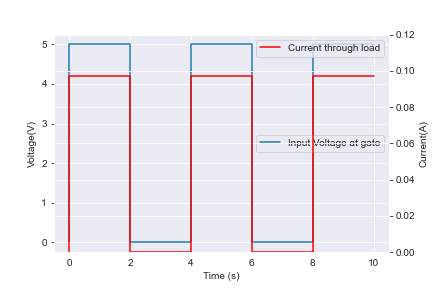
\includegraphics[width=1\linewidth]{./Figures/NMOS.png}
		    \caption{} \label{subfig:fig3}
     \end{subfigure}
     \begin{subfigure}[]{0.3\textwidth}
             \centering
  		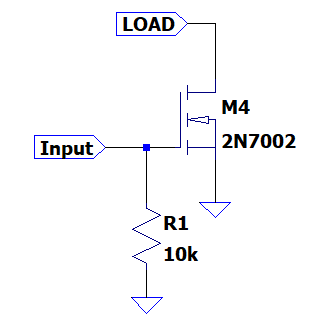
\includegraphics[width=1\linewidth]{./Figures/circNMOS.png}
		   \caption{ } \label{subfig:fig4}
     \end{subfigure}
   \caption[{Fuse Characteristics}]{NMOS final Results   (a)  LT Spice simulation (b) Basic Circuit }
    \label{fig:two}
 \end{figure}




\vfill


\chapter{Bidirectional current measurement}\label{ch:bidircurrent}
%**********************************************
\section{Overview}
In figure \ref{fig:block} the highlighted blocks were added into the previous structure, the blocks highlighted in red are covered in this report. The current sense circuitry was added at its position after the load so that the current it will measure is the current discharging from the battery or charging into the battery. The current sense amplifier will be used to produce a voltage between 0V and 5V that will correspond proportionally to the current in a designed range of 3V. The load can also be connected and disconnected with the help of the designed low side switch.


\begin{figure}[!htb]
\centering
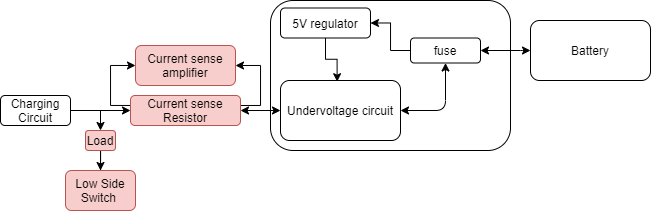
\includegraphics[scale=0.5]{./Figures/block}
\caption{Block Diagram showing circuit structure}
\label{fig:block}
\end{figure}

\subsection{Literature}
The bidirectional current sense amplifier is an op amp that is setup internally as can be seen in figure \ref{fig:data}. This internal circuitry is necessary because the resistors used need to be very accurate in order for current sensing to be accurate \cite{utube}. Another reason that the tsc213 is being used over a conventional op amp is because this device has a absolute differential voltage of 26V and a common mode voltage range of $gnd-0.3V$ to 26V. This is important for us because we can have differential voltages of up to 7.2V ($7.2-0$) and common mode voltages of about 7.2V which would not work with the previously used MCP op amp. The current sense amplifier will have its positive and negative inputs connected across a shunt resistor, the current sense amplifier will then amplify this difference by 50 (refer to \ref{fig:data}).


\subsection{Design}
When designing the current sense amplifier the current range that will be used should be considered. The most current that should be discharged from the battery should be 100mA. The maximum that the battery should charge at is 400mA. The current range was then determined to be $-150mA<I_{range}<450mA$, the additional 50mA was added as a safety factor to ensure the tsc213 does not breach the 0-5V output range. The output voltage range will be dependant on the differential voltage of the op amp and the reference voltage chosen (refer to eq \ref{eq:refeq}). The differential voltage will be dependant on the shunt resistance and the current through the shunt.
\begin{equation}
    V_o=(R_{shunt}\times I_{shunt})\times50+V_{REF}
    \label{eq:refeq}
\end{equation}
Using eq.\ref{eq:refeq} $R_{shunt}$ is designed to give an output voltage swing of 3V.
\begin{center}
    $V_{swing}=((R_{shunt}\times 0.45)-(R_{shunt}\times -0.15))\times 50$. \ \ $R_{shunt}=0.1$\textohm 
\end{center}
This results in voltage range across the shunt of $-15mV<V_{shunt}<45mV$. With a 0V at $V_{ref}$ the output range (using eq.\ref{eq:refeq}) would be -0.75V to 2.25V. This is not within 0V to 5V, this is where $V_{ref}$ is used to place the output voltage into a desirable range. The minimum $V_{ref}$ to get the output into the desired range would be 0.75V. The maximum $V_{ref}$ that would place the maximum output voltage at 5V would be 2.75V (i.e. 5-2.25). The average of the maximum and minimum $V_{ref}$ is then taken and found to be 1.75V. By doing this output voltage will be equally far from the upper and lower bounds of the 0V to 5V specification. To achieve this 1.75V the voltage from a 5V regulator is divided with resistors (refer to figure \ref{fig:circ}). \newline

To reduce the noise at the output a low pass filter was designed and placed at the output of the TSC213. 
\begin{equation}
    f_c=\frac{1}{2\pi RC}
    \label{eq:f}
\end{equation}
Using equation \ref{eq:f} and designing for 50Hz cutoff with a chosen resistor of 1.5k\textohm  \cite{lowpass}. For the chosen resistance a capacitance of 2.2\textmicro F was calculated. The reason 50Hz is designed for is because that is the frequency of noise that the 12V wall plug introduces into the circuit. 

\begin{figure}[!htb]
\centering
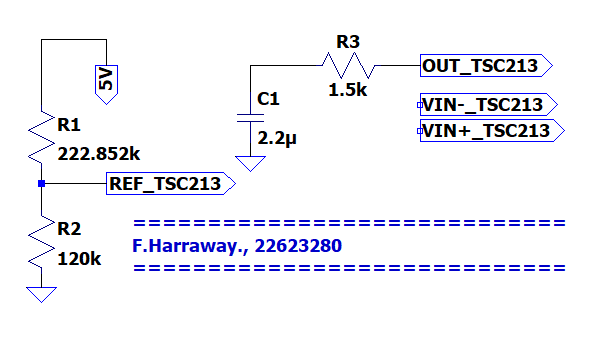
\includegraphics[scale=0.45]{./Figures/circ.png}
\caption{Oscilloscope Measurements}
\label{fig:circ}
\end{figure}

\newpage
\section{Results}

 \begin{figure}[!htb]
 \footnotesize
 \centering
    \begin{subfigure}[]{0.48\textwidth}
              \centering
  		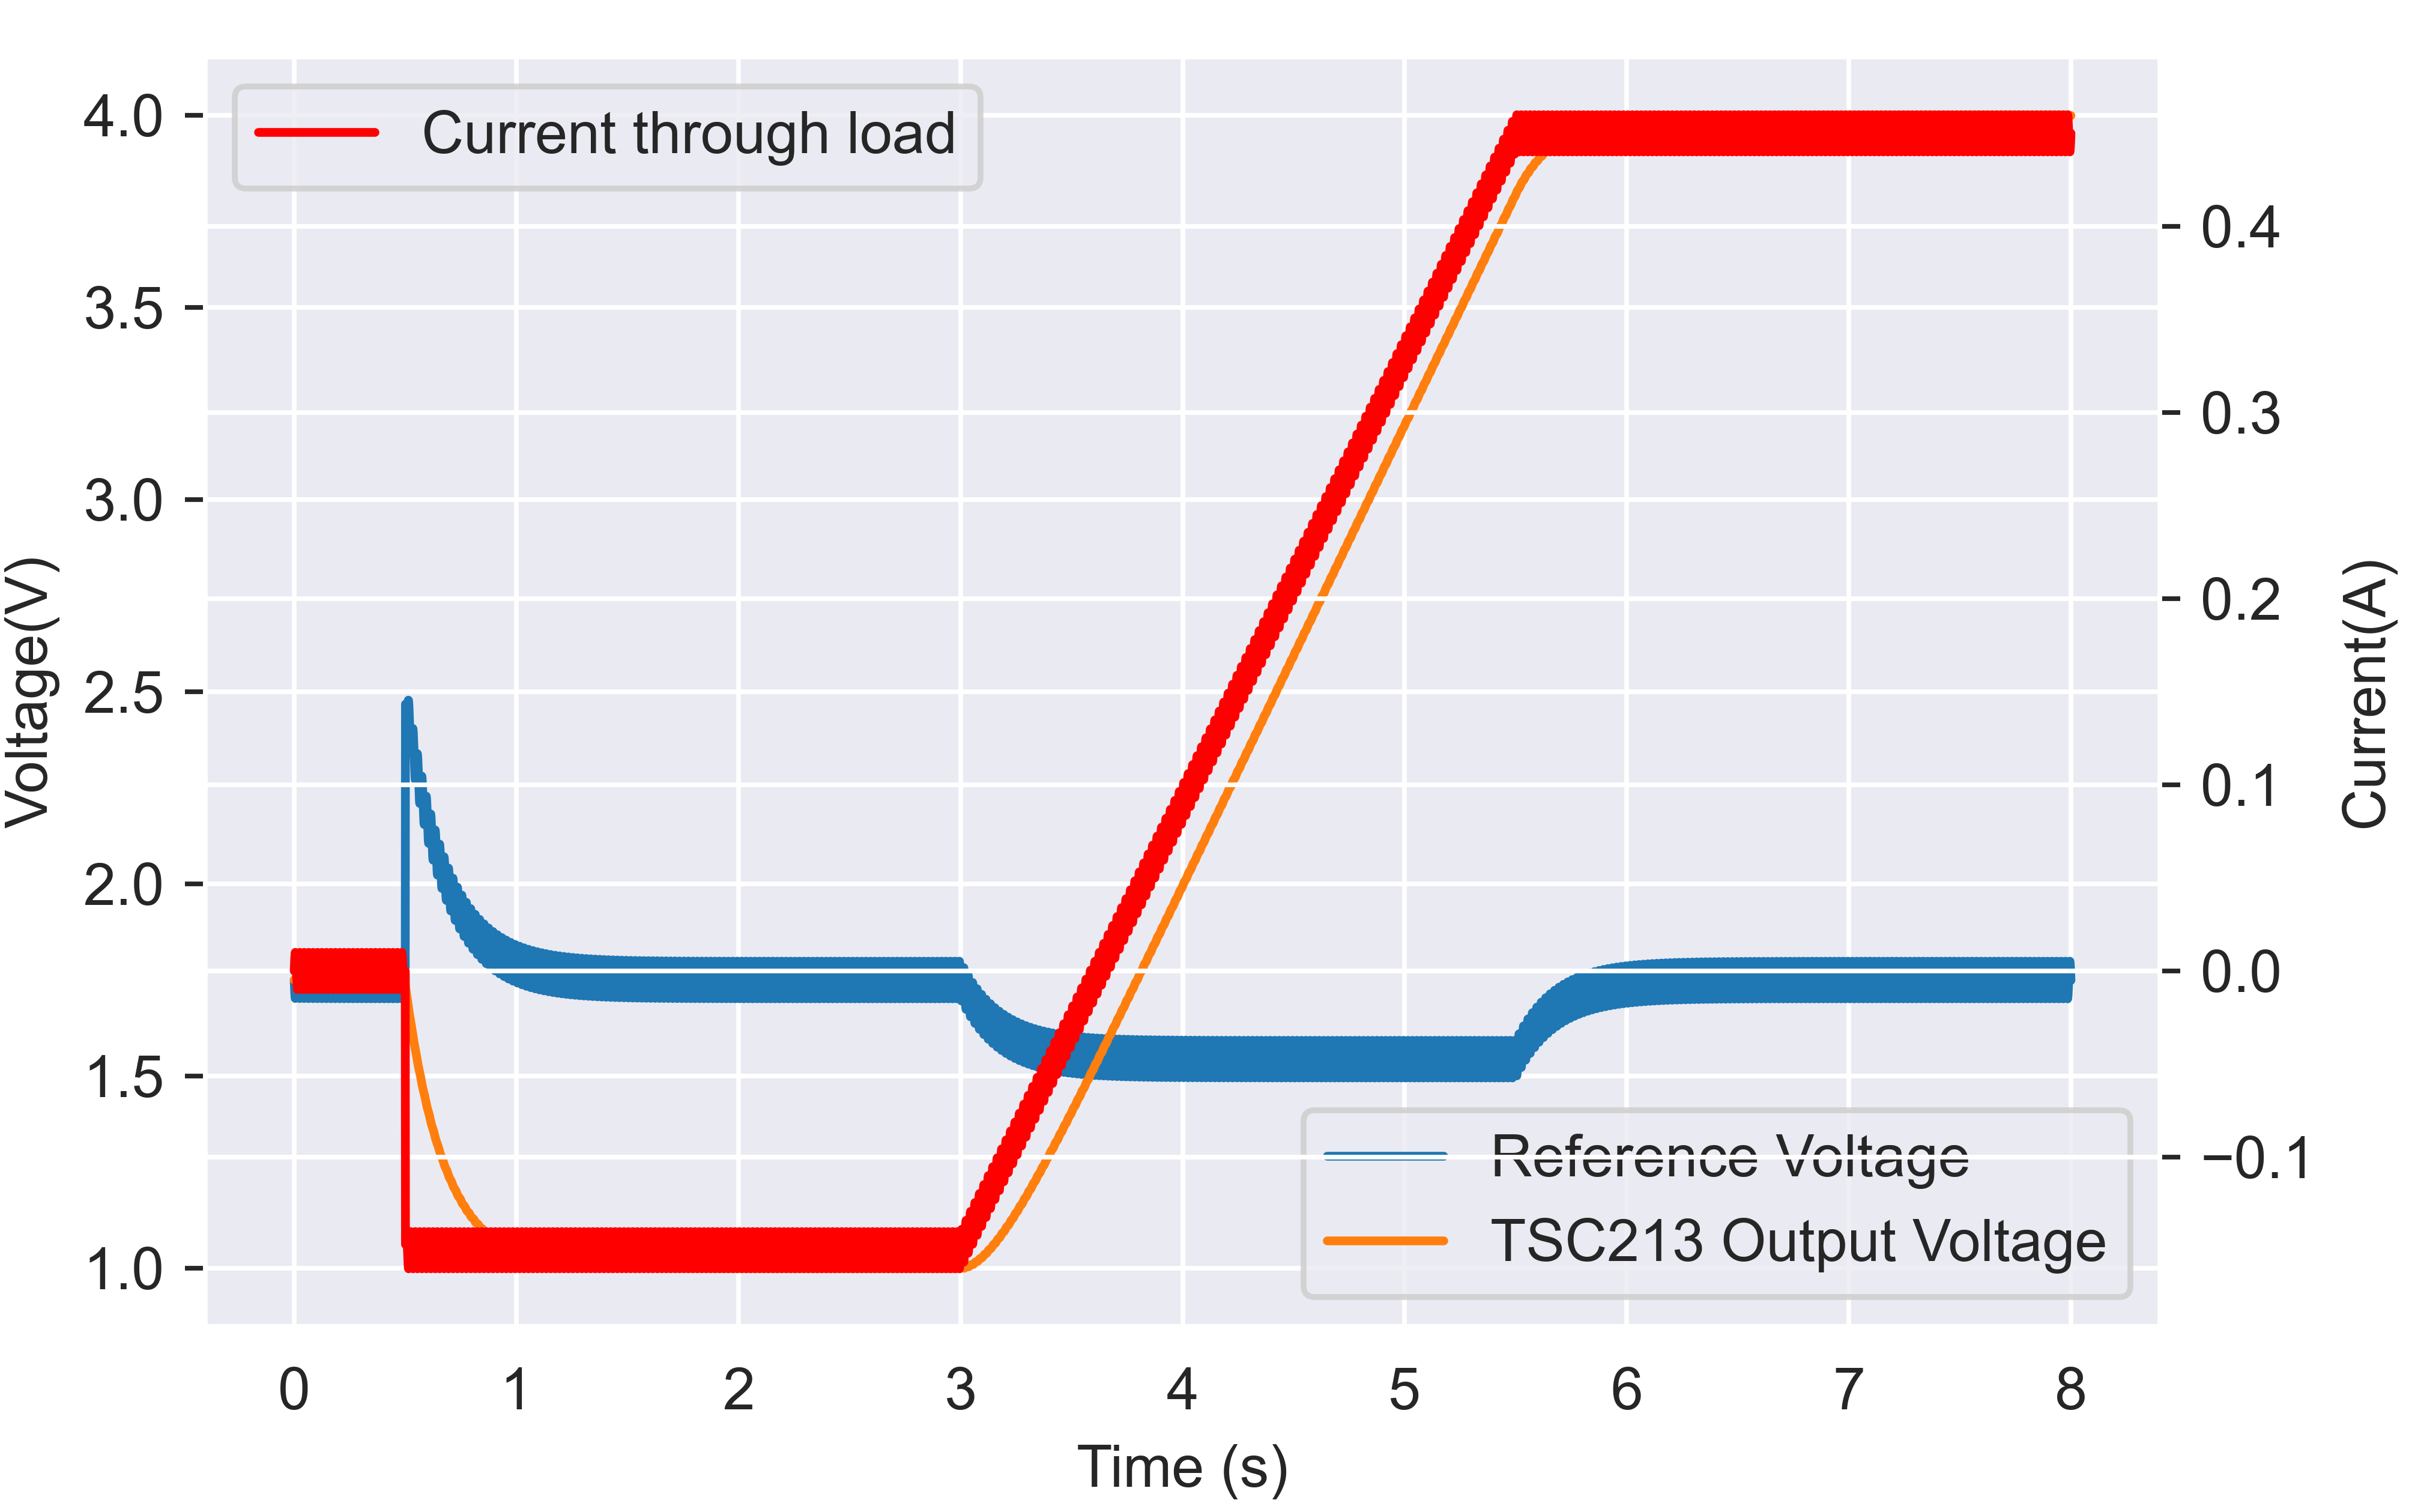
\includegraphics[width=1\linewidth]{./Figures/circuit.png}
		    \caption{} \label{subfig:sim}
     \end{subfigure}
     \begin{subfigure}[]{0.5\textwidth}
             \centering
  		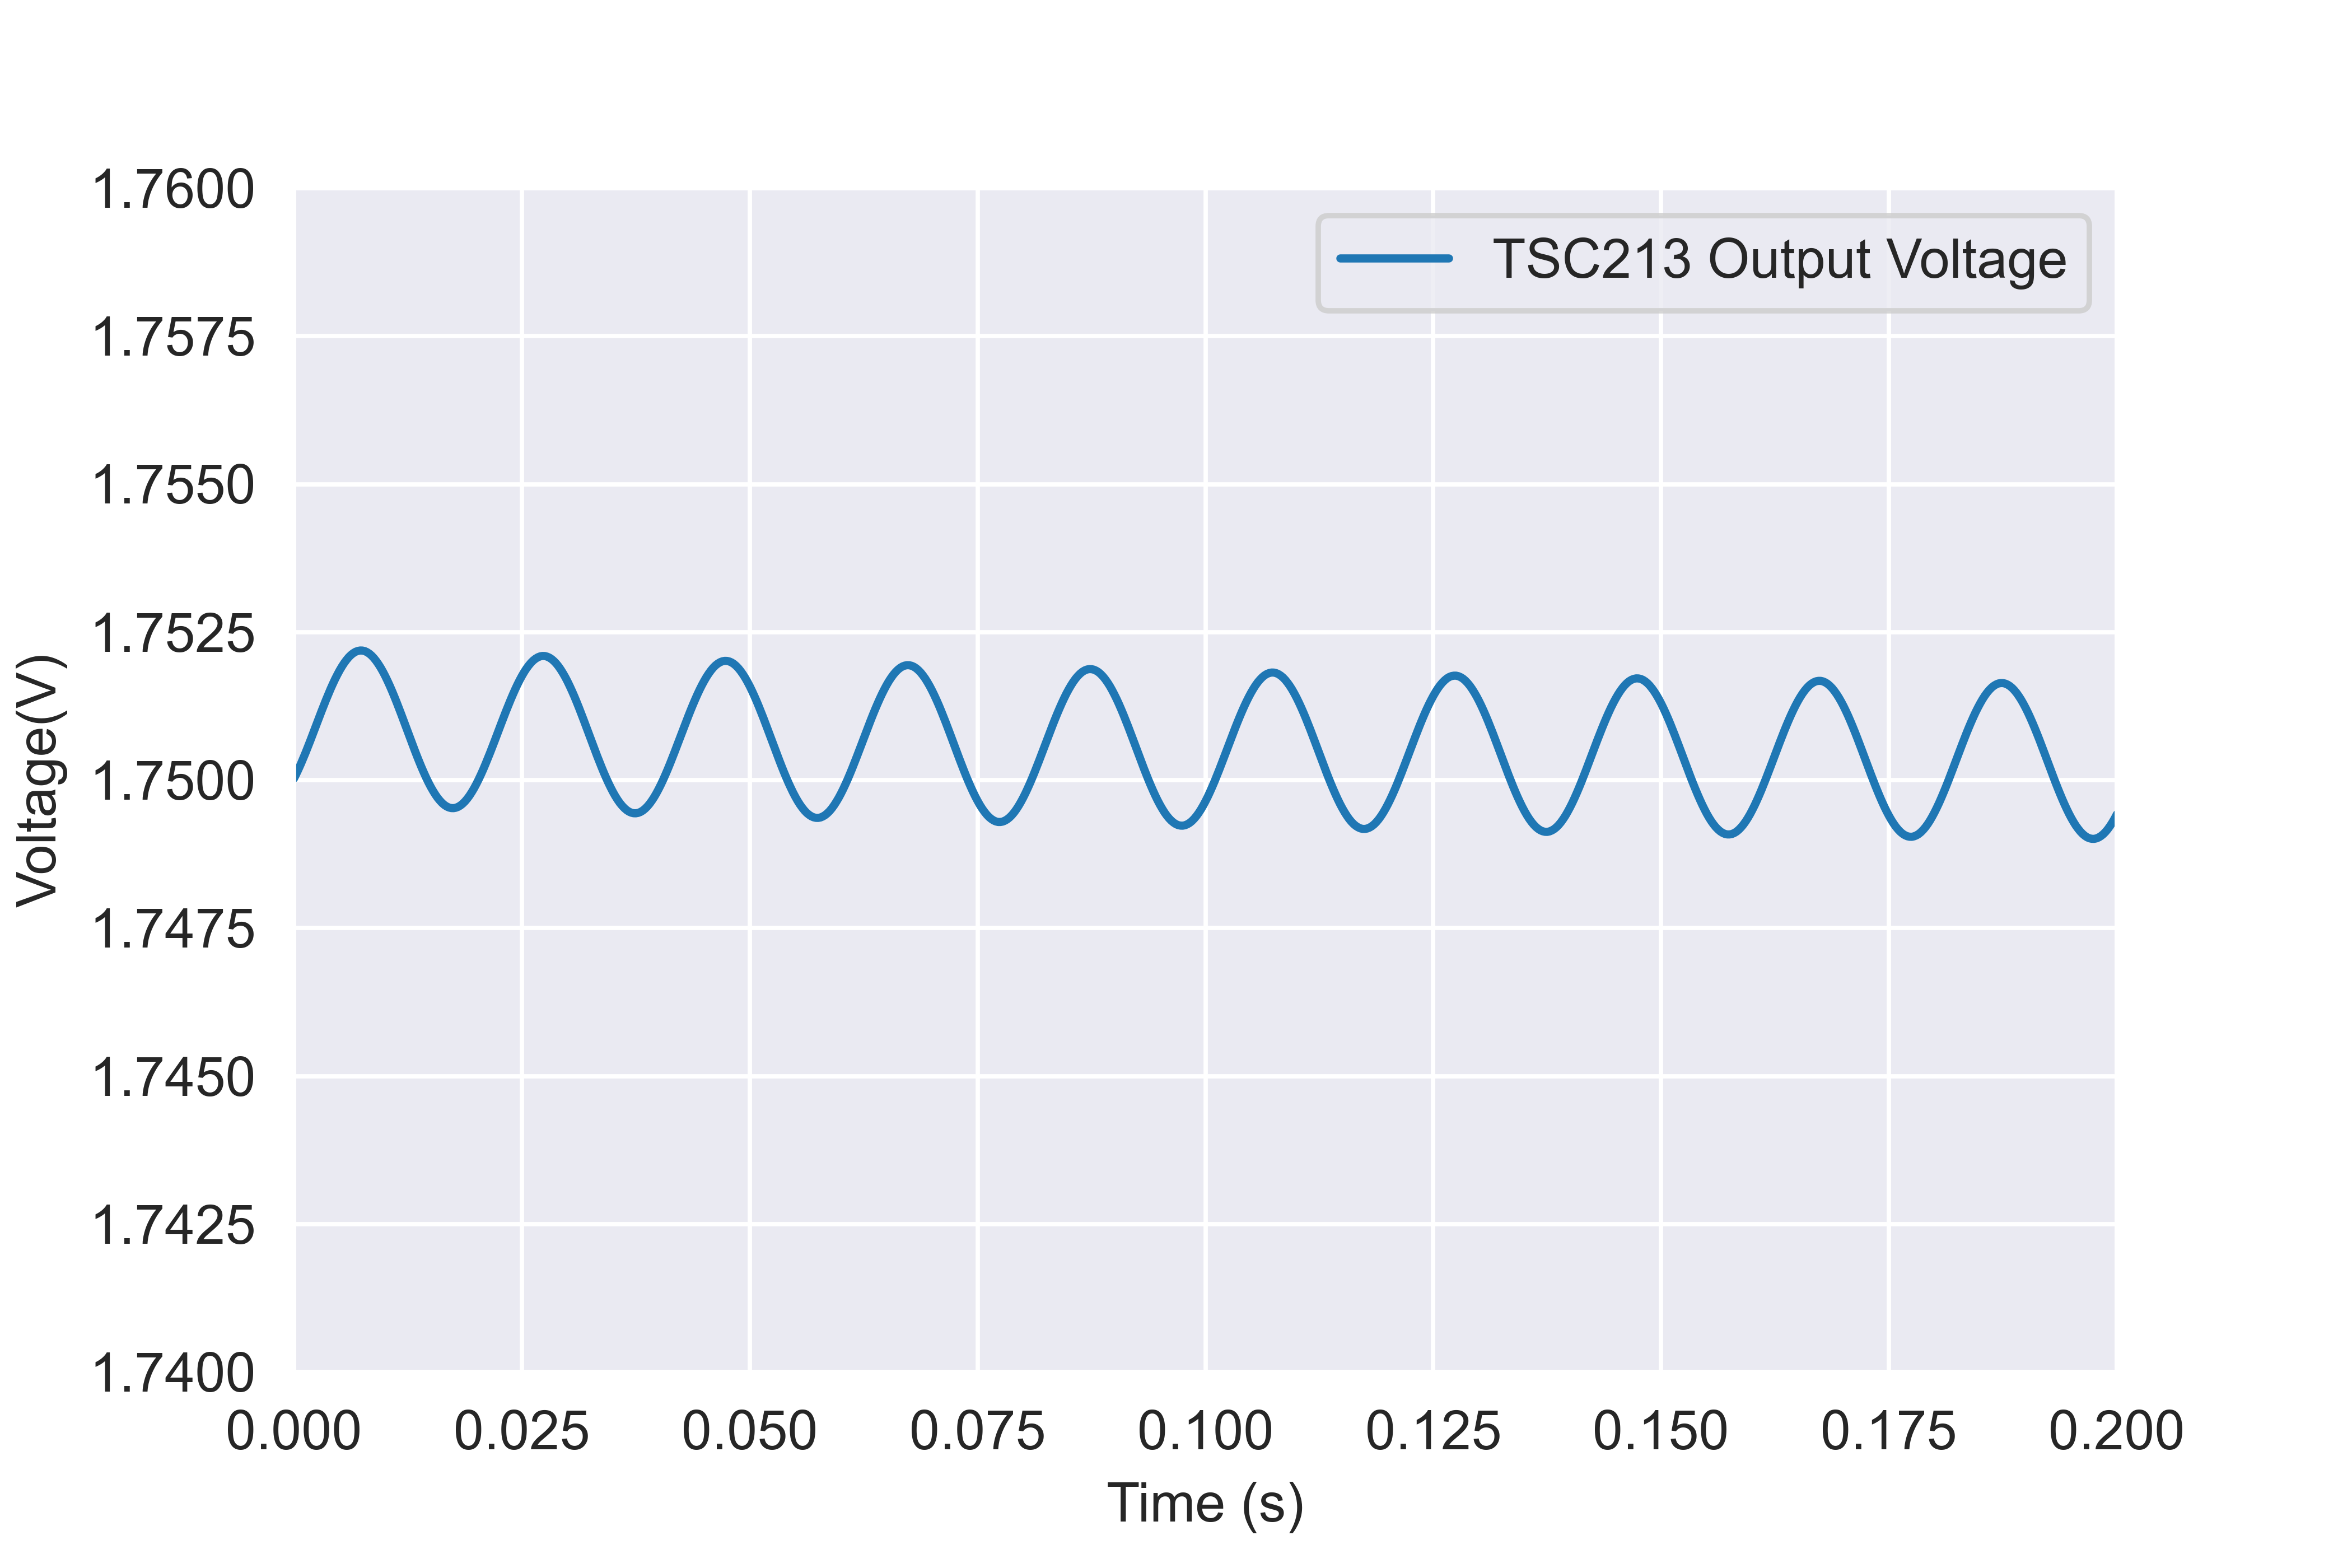
\includegraphics[width=1\linewidth]{./Figures/noise.png}
		   \caption{ } \label{subfig:noise}
     \end{subfigure}
   \caption[{Spice}]{LT Spice results   (a)  Simulation results (b)Noise in output signal }
 
 \end{figure}


\begin{figure}[!htb]
\centering
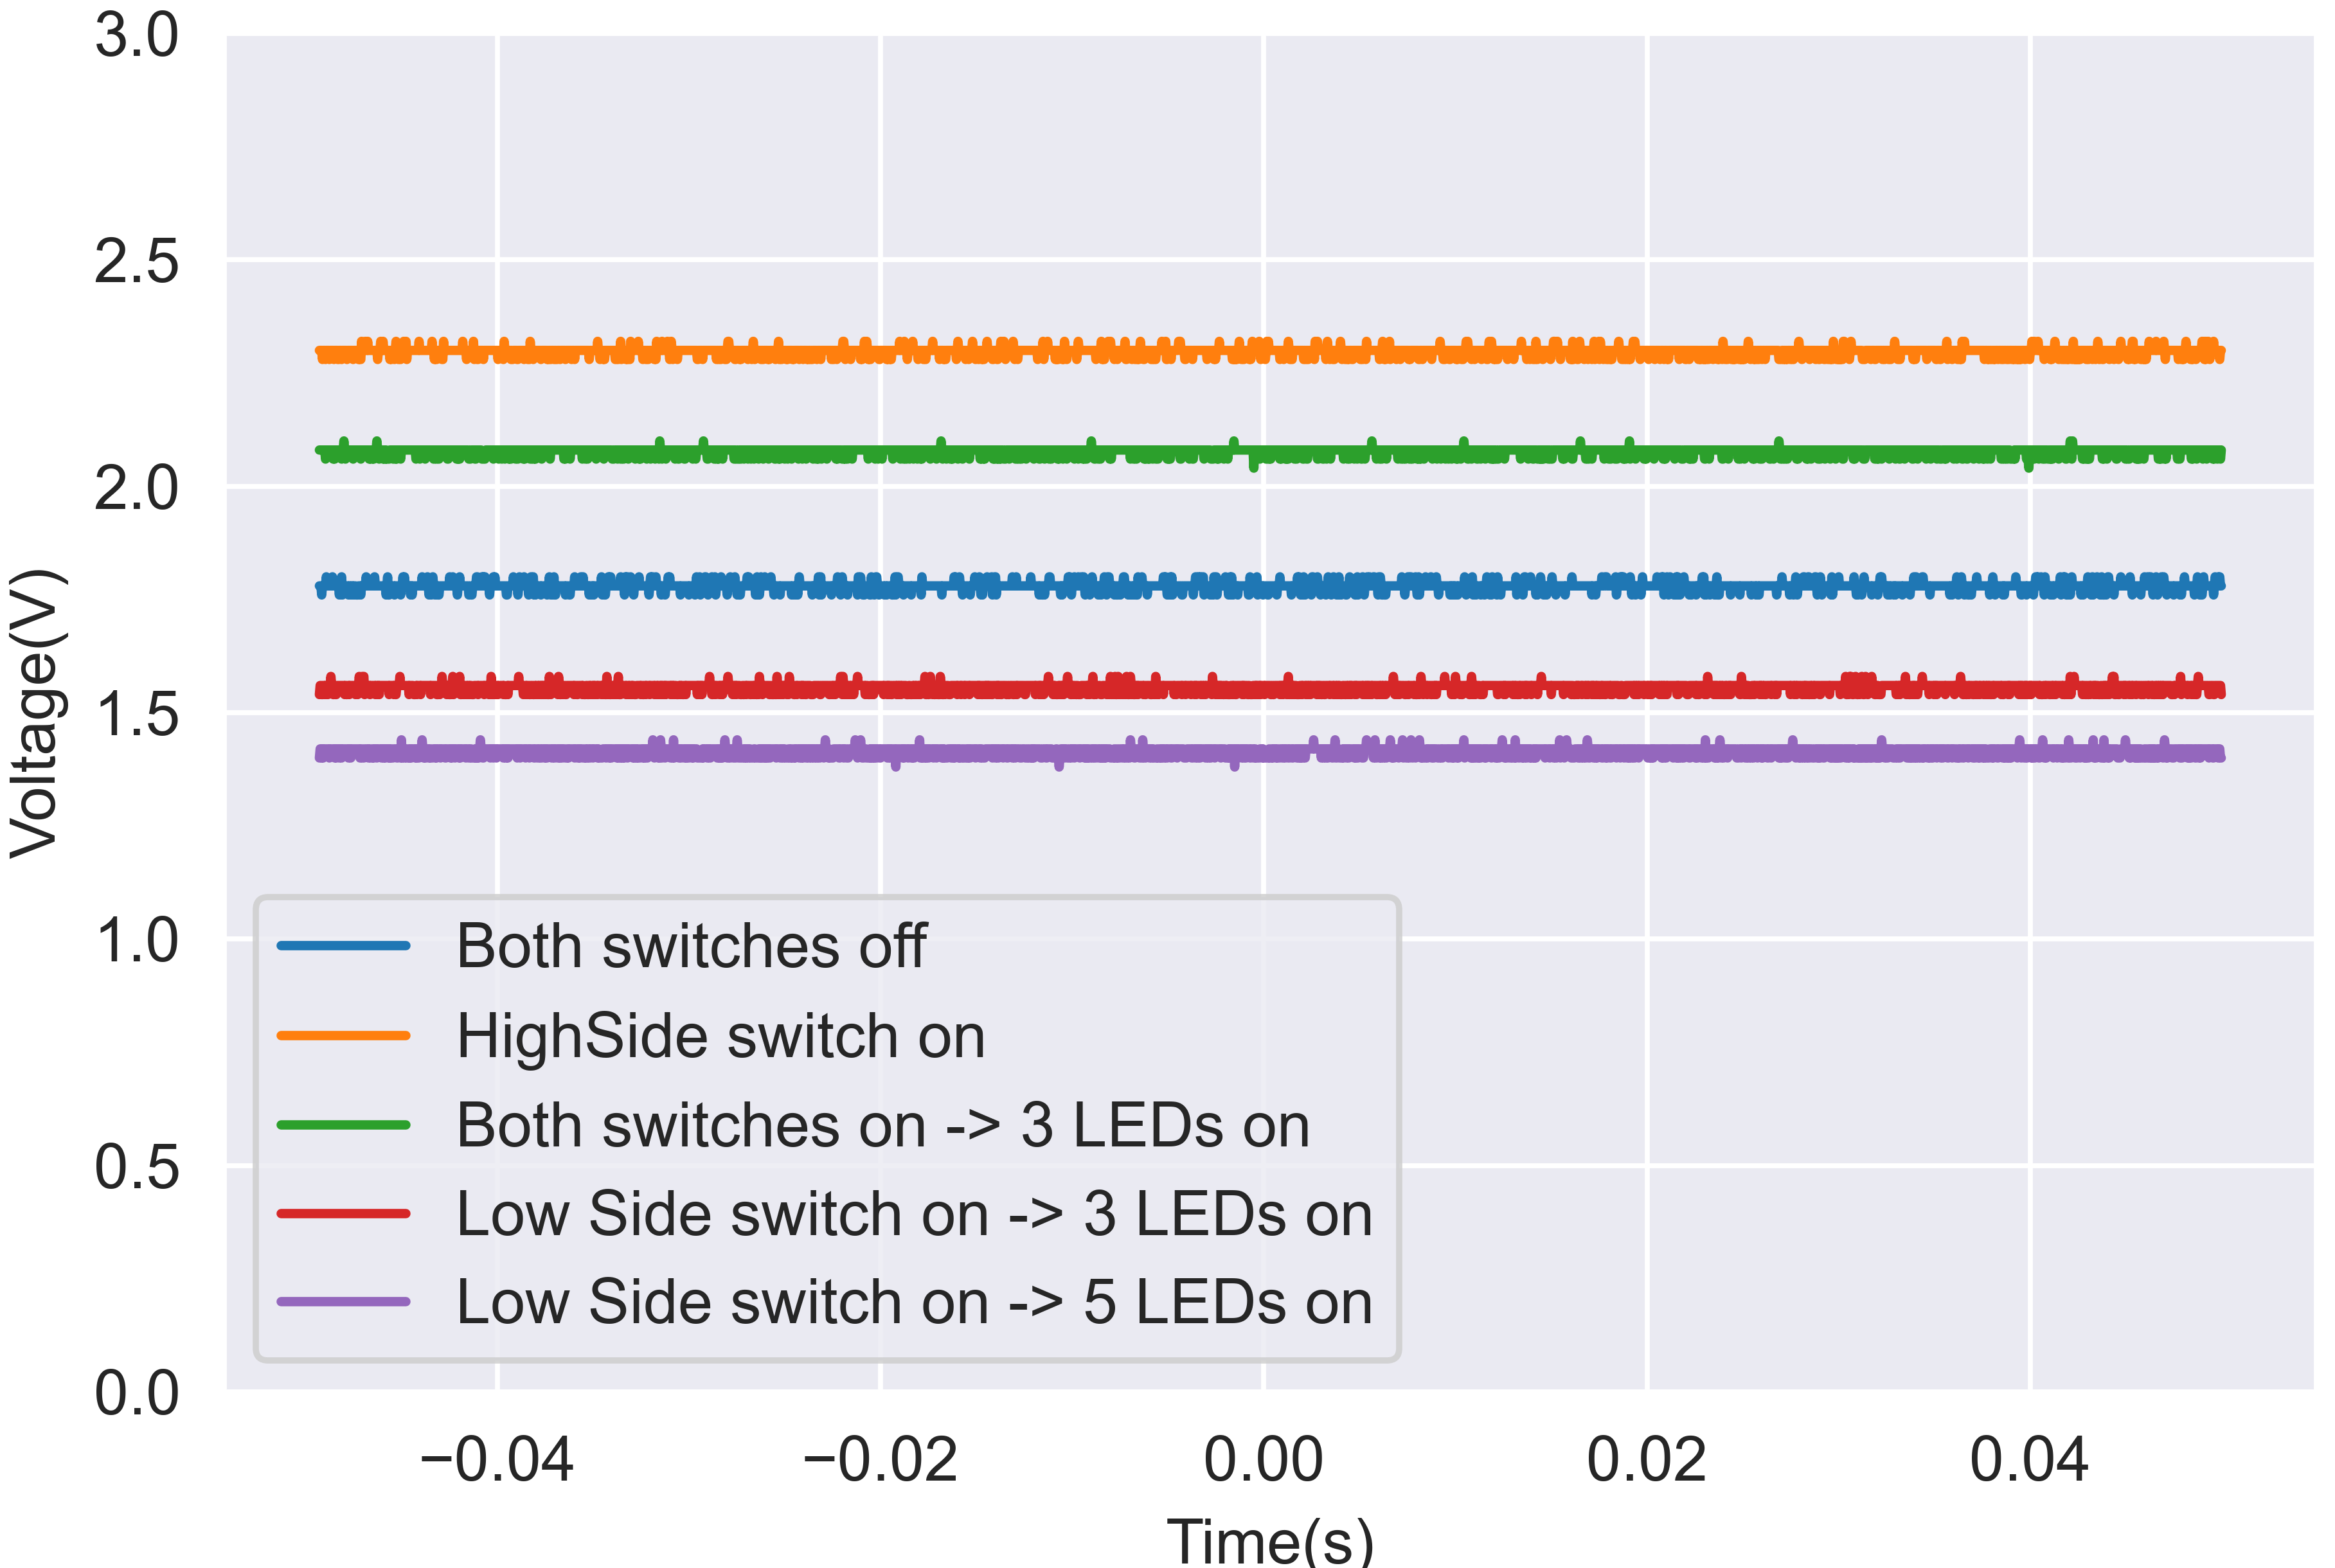
\includegraphics[scale=0.7]{./Figures/meas.png}
\caption{Oscilloscope Measurements}
\label{fig:meas}
\end{figure}

\begin{table}[!htb]
        \centering
        \footnotesize
        \caption{Resistor measurements}
         \begin{tabular}{lrrrr}
          \toprule
             & $Resistor \ Voltage$ & $Calculated \ Current$ \\
             &  [V]  & [mA]\\
          \midrule
         R1      & 3.35 & 15.23 \\
          R2 & 3.34   & 15.18 \\
          R3       &3.36 & 15.27 \\
          R4        &3.35 & 15.23 \\
          R4        &3.37 &15.32 \\
          \bottomrule
        \end{tabular}
     \label{tab:PVresults}
\end{table}
The LT spice simulations(figure \ref{subfig:sim}) show the output working correctly and the noise( figure \ref{subfig:noise}) is within spec. The measured noise on the output of the TSC213 was found to be 40mV ($V_{PK-PK}$) on the oscilloscope, however in the past I have found that oscilloscopes are not particularly accurate for these types of measurements. The general oscilloscope results are promising ( figure \ref{fig:meas}). The current through the LEDs is slightly less than 20mA as can be seen in table \ref{tab:PVresults}.
\vfill



\include{Chapter3}
\include{Chapter4}
\include{Chapter5}
\include{Chapter6}


% Bibliography
\bibliography{References}

% End matter
\appendix
\chapter{GitHub Activity Heatmap}
\makeatletter\@mkboth{}{Appendix}\makeatother
\label{appen:github_heatmap}


     \begin{figure}[!htb]
     \centering
     	\fbox{\includegraphics[width=1\linewidth]{./Figures/gitHub.png}}
	\label{fig:github}
	\end{figure}
     \chapter{Data sheet info}

\begin{figure}[!htb]
\centering
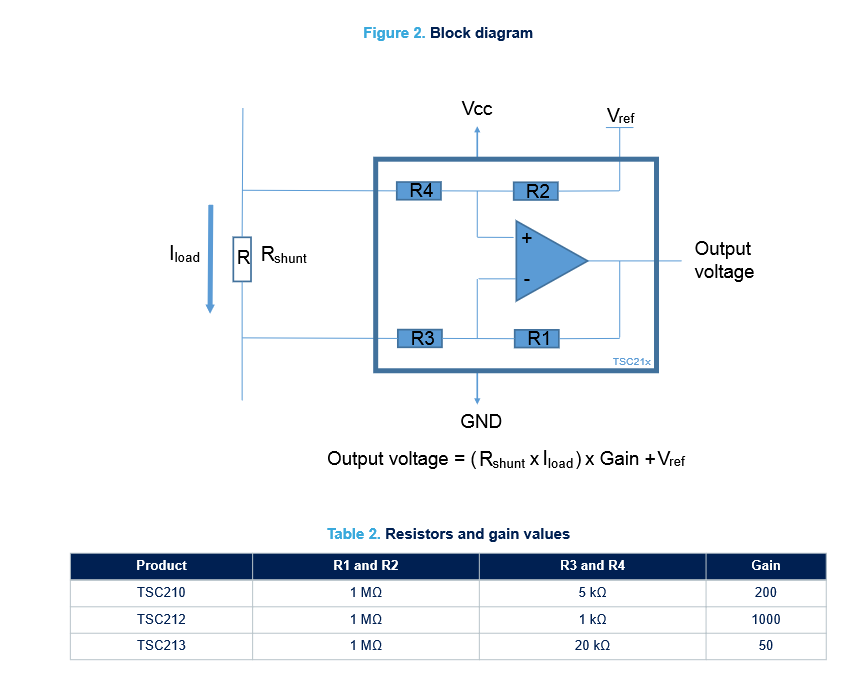
\includegraphics[scale=0.5]{./Figures/datasheet}
\caption{tsc213 data sheet information}
\label{fig:data}
\end{figure}


\begin{figure}[!htb]
\centering
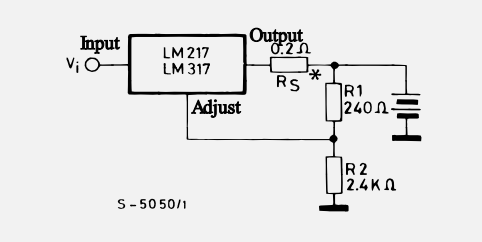
\includegraphics[scale=0.35]{Figures/circuitSTM.png}
\caption{Application Circuit For LM317\cite{STM}}
\label{fig:app}
\end{figure}




\begin{table}[!htb]
        \centering
        \footnotesize
        \caption{Thermal Resistance Values \cite{sink}\cite{STM}}
         \begin{tabular}{lrrrr}
          \toprule
             & $Thermal Resistance$ \\
             &  [\textdegree C/W] \\
          \midrule
          $\theta_{j-c}$ & 5      \\
          $\theta_{s-a}(worst case)$ &  20     \\
          $\theta_{j-a}$ &  50     \\

          \bottomrule
        \end{tabular}
     \label{tab:Thermal values}
\end{table}


\chapter{Additional Info}
\begin{figure}[!htb]
\centering
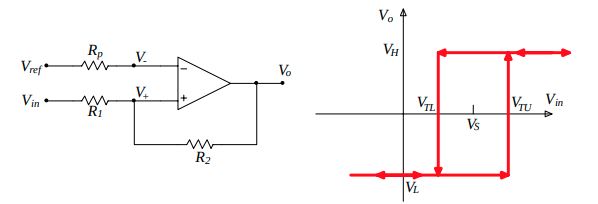
\includegraphics[scale=0.7]{./Figures/schmidt}
\caption{Non inverting Schmidt trigger\cite{Schmidt}}
\label{fig:schmidt}
\end{figure}




\end{document}

